\documentclass{beamer}
\usepackage[french]{babel}
\usepackage[T1]{fontenc}
\usepackage[utf8]{inputenc}
\usepackage{listings}
\usepackage{color}

\definecolor{Gray}{RGB}{245,245,245}
\definecolor{CPPGray}{RGB}{120,120,120}

\lstdefinestyle{default}{
  showspaces=false,
  showtabs=false,
  breaklines=true,
  showstringspaces=false,
  breakatwhitespace=true,
  basicstyle=\ttfamily,
  backgroundcolor=\color{Gray},
  numbers=left, numbersep=3pt, stepnumber=1, numberstyle=\tiny\color{CPPGray},
  rulecolor=\color{CPPGray},
  basicstyle=\tiny
}

\definecolor{dkblue}{rgb}{0,0,.6}

\lstset{language=php,
  keywordstyle = \color{dkblue},
  style=default}
  
\lstdefinelanguage{behat}{
    keywords={Feature,Background,Scenario,Given,When,Then,And}
}
\lstset{language=behat,
  keywordstyle = \color{dkblue},
  style=default}

\newcommand{\GT}[1]{\alert{\emph{#1}}}

\usetheme{Frankfurt}

%\setbeamertemplate{mini frames}{}
% GT: Symboles de navigation pas vraiment utiles: je ne les ai jamais utilises!!
\setbeamertemplate{navigation symbols}{}

\title[Pr\'esentation du projet de ma\^itrise]{D\'eveloppement d'un module d'extension Moodle d'aide \`a la correction de questions\\de type \og texte long \fg{} }
\author{Philippe Girard}
\institute{Universit\'e du Qu\'ebec \`a Montr\'eal}
\date{26 juin 2018}

\begin{document}
  \begin{frame}[plain]
    \titlepage
  \end{frame}
  
  \begin{frame}[plain]
    \tableofcontents[hideallsubsections]
  \end{frame}
  
  \section[Introduction]{Motivation initiale du projet}
  \begin{frame}
    \frametitle{Motivation initiale du projet}

    \begin{block}{Id\'ee de d\'epart}
      Magda Fusaro~: cours avec de nombreux petits travaux 
    \end{block}

    \vfill

    \begin{block}{Objectif}
      \begin{itemize}
        \item Aider \`a la correction de <<textes (courts) \`a d\'eveloppement>>
      \end{itemize}
    \end{block}

    \vfill

    \begin{block}{Contrainte}
      \begin{itemize}
        \item Microsoft Word ou Moodle
      \end{itemize}
    \end{block}
    \vfill
  \end{frame}
  
  \begin{frame}
    \frametitle{\insertsection}
    \begin{block}{Fonctionnalit\'es}
      \begin{itemize}
        \item Mise en \'evidence \alert{de mots-cl\'es}
        \item[]
        \item Affichage de la r\'eponse de l'enseignant \`a c\^ot\'e de celle de l'\'etudiant
        \item[]
        \item Fonctionnement en fran\c{c}ais et en anglais
      \end{itemize}
    \end{block}
  \end{frame}
  
  \section[Moodle]{Moodle et son architecture modulaire}
  \begin{frame}
    \frametitle{\insertsection}

    \begin{block}{Moodle}
      \begin{itemize}
        \item \textit{Learning Management System} (LMS)
      \end{itemize}
    \end{block}

    \vfill

    \begin{block}{Principales caract\'eristiques}
      \begin{itemize}
        \item Modulaire: 
        \begin{itemize}
          \item Cours 
          \item Sections
          \item  Activit\'es
        \end{itemize}
        \item Logiciel libre
      \end{itemize}
    \end{block}
    \vfill
  \end{frame}
  
  \begin{frame}
    \frametitle{\insertsection}
  
    \begin{block}{Permet la  cr\'eation de formulaires en ligne}
    \end{block}
  
    \vfill
  
    \begin{block}{Permet diff\'erents types de questions}
      \begin{itemize}
        \item Choix multiples
        \item R\'eponse courte
        \item Num\'erique
        \item Question Cloze
        \item Composition
      \end{itemize}
    \end{block}
    \vfill
  \end{frame}
  
  \begin{frame}
    \frametitle{\insertsection}
    \begin{block}{Les modules d'extensions Moodle}
      \begin{itemize}
        \item Rapport de questionnaire (\textit{Quiz report})
        \item Type de question (\textit{Question type})
        \item Comportement de question (\textit{Question behaviour})
      \end{itemize}
    \end{block}
  \end{frame}
  
  \section[Mots-cl\'es]{D\'etection et analyse des mots-cl\'es}
  \begin{frame}
    \frametitle{\insertsection}
    \begin{block}{Lemmatisation}
      \begin{itemize}
        \item Trouve le lemme d'un mot
              \begin{itemize}
                      \item Lemme = Forme \alert{canonique} d'un mot
                      \item Exemple: aimerait $\Rightarrow$ aimer
                      \end{itemize}

       \medskip
       \item Aucune biblioth\`eque PHP fran\c{c}ais/anglais
      \end{itemize}
    \end{block}
  
    \vfill
    \pause
  
    \begin{block}{Racination (\textit{stemming})}
      \begin{itemize}
        \item Trouve le radical (\textit{stem}) d'un mot
        \begin{itemize}
        \item Radical = Racine du mot
        \item Exemple: aimerait $\Rightarrow$ aim
        \end{itemize}

       \medskip
        \item \texttt{php-stemmer}: biblioth\`eque multilingue PHP
      \end{itemize}
    \end{block}
    \vfill
  \end{frame}
  
  \begin{frame}
    \frametitle{\insertsection}
    \begin{block}{\texttt{php-stemmer}}
      Traduction PHP des algorithmes Snowball
    \end{block}
  
    \vfill
  
    \begin{block}{Snowball}
      \begin{itemize}
        \item D\'evelopp\'e par Martin Porter
        \item Language de traitement de texte
        \item Compile en C ou en Java
        \item Algorithmes de racination pour 12 langues, dont le fran\c{c}ais
      \end{itemize}
    \end{block}
    \vfill
  \end{frame}
  
  \section[Tests]{Tests pour int\'egration \`a Moodle d'un module d'extension}
  \begin{frame}
    \frametitle{\insertsection}
    \begin{block}{Environnement de tests}
      Machine virtuelle Xubuntu
      \smallskip

      PHP 7.0.22 
      \smallskip
      
      MySQL 5.7.20
      \smallskip

      Moodle 3.4 install\'e avec Git
    \end{block}
  \end{frame}
  
  \begin{frame}
    \frametitle{\insertsection}
    \begin{block}{Tests unitaires}
      V\'erifications \`a petite \'echelle (m\'ethodes)
  
      D\'ependances remplac\'ees par des \textit{stubs}
  
      Ex\'ecut\'es avec \textit{PHPUnit}
    \end{block}
  
    \vfill
  
    \begin{block}{Ex\'ecution des tests unitaires}
      8750 tests, 90 575 v\'erifications
      \medskip

      8682 \textit{success}, 67 \textit{skipped} et 1 \textit{failure}:
      \begin{itemize}
        \item Encodage de la base de donn\'ees UTF8 non sensible \`a la casse
      \end{itemize}
    \end{block}
  \end{frame}
  
  \begin{frame}
    \frametitle{\insertsection}
    \begin{block}{Tests d'acceptation}
      Tests automatis\'es --- de bout en bout
  
      Tests \textit{behat} ex\'ecut\'es avec \textit{Selenium}
    \end{block}
  
    \vfill
  
    \begin{block}{Ex\'ecution des tests d'acceptation}
      1 771 sc\'enarios et 43 824 \'etapes

      \medskip

      4 sc\'enarios et 102 \'etapes ignor\'es

      \medskip
      6 sc\,énarios et 6 \'etapes \'echou\'es:
      {\footnotesize
      \begin{itemize}
        \item Un \'etudiant passe d'une activit\'e \`a une autre
        \item Filtre du calendrier mensuel
        \item Navigation entre les modes de groupes
        \item Solr non install\'e (2 erreurs)
        \item L'enseignant ne voit pas quels \'etudiants sont actifs
      \end{itemize}
    }
    \end{block}
    \vfill
  \end{frame}
  
  \section[Mise en oeuvre]{Mise en oeuvre et tests du module d'extension \texttt{qtype\_essayhelper}}
  \begin{frame}
    \frametitle{\insertsection}
    \begin{block}{Fonctionnalit\'es du module d'extension \texttt{qtype\_essayhelper}}
      Module d'extension bas\'e sur \texttt{qtype\_essay}
    \end{block}
  \end{frame}
  
  \begin{frame}
    \frametitle{\insertsection}
    \begin{block}{Fonctionnalit\'es retir\'ees}
      \begin{itemize}
        \item \'Edition de texte \textit{WYSIWIG}
        \item Remise de fichiers
      \end{itemize}
    \end{block}
    
    \vfill
  
    \begin{block}{Fonctionnalit\'es conserv\'ees}
      \begin{itemize}
        \item R\'etroaction g\'en\'erale
        \item Mod\`ele de r\'eponse
        \item Information de l'\'evaluateur
      \end{itemize}
    \end{block}
    
    \vfill
  
    \begin{block}{Fonctionnalit\'es ajout\'ees}
      \begin{itemize}
        \item Mots-cl\'es
        \item R\'eponse officielle de l'enseignant
        \item Langue de racination
      \end{itemize}
    \end{block}
    \vfill
  \end{frame}
  
  \begin{frame}
  \frametitle{\insertsection}

\begin{columns}
\begin{column}{0.38\textwidth}
 \alert{Structure des fichiers~$\Rightarrow$}
\end{column}
\begin{column}{0.6\textwidth}
\vspace*{-1cm}
  \begin{center}
    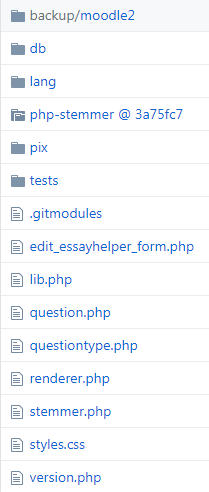
\includegraphics[scale=0.6]{../images/architecture.png}
  \end{center}
\end{column}
\end{columns}

  \end{frame}
  
  \begin{frame}
  \frametitle{\insertsection}
  \alert{Principales classes}
\vfill
    \hspace*{-0.75cm}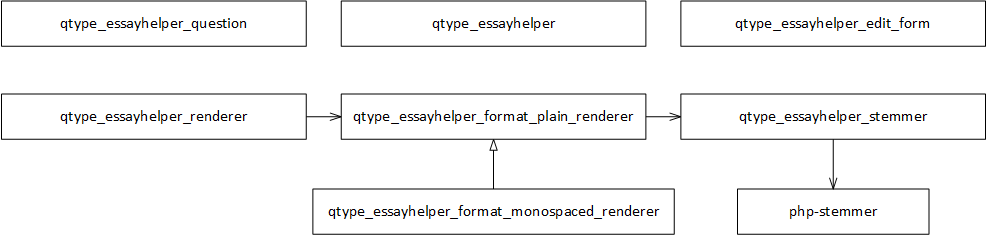
\includegraphics[scale=0.475]{../images/class-simple.png}
  \end{frame}
  
  \begin{frame}[plain]
  %\frametitle{\insertsection}
    \begin{center}
    \hspace*{-0.9cm}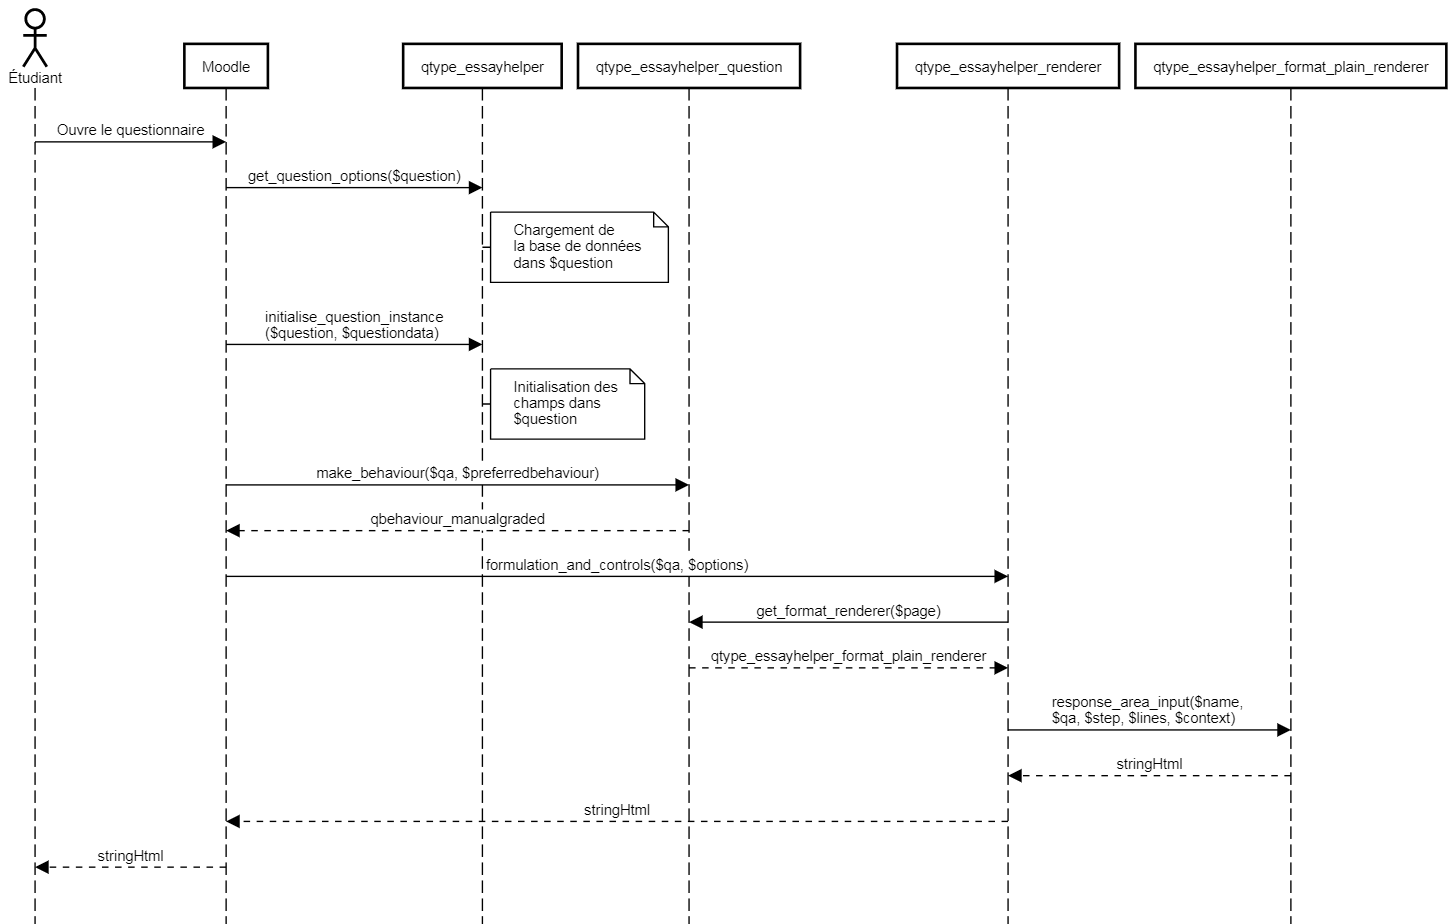
\includegraphics[scale=0.245]{../images/diagramme-flux.png}
    \end{center}
  \end{frame}
  
  \begin{frame}[fragile,plain]
    %\frametitle{\insertsection}
    \alert{Exemple de test d'acceptation \'ecrit avec \texttt{behat}}
\begin{lstlisting}[language=behat,frame=l,numbers=none,basicstyle=\footnotesize]
@qtype @qtype_essay
Feature: Test creating an Essay question
  As a teacher
  In order to test my students
  I need to be able to create an Essay question

  Background:
    Given the following "users" exist:
      | username | firstname | lastname | email               |
      | teacher1 | T1        | Teacher1 | teacher1@moodle.com |
    And the following "courses" exist:
      | fullname | shortname | category |
      | Course 1 | C1        | 0        |
    And the following "course enrolments" exist:
      | user     | course | role           |
      | teacher1 | C1     | editingteacher |
    And I log in as "teacher1"
    And I am on "Course 1" course homepage
    And I navigate to "Question bank" node in "Course administration"
\end{lstlisting}
\end{frame}
 
 \begin{frame}[fragile,plain]
    %\frametitle{\insertsection}
\begin{lstlisting}[language=behat,frame=l,numbers=none,basicstyle=\footnotesize]
Scenario: Create an Essay question with Response format set to 'HTML editor'
  When I add a "Essay" question filling the form with:
   | Question name    | essay-001                |
   | Question text    | Write a 500 word essay.  |
   | General feedback | This is general feedback |
   | Response format  | HTML editor              |
  Then I should see "essay-001"

  [...]
\end{lstlisting}
\end{frame}
  
  \section[R\'esultats]{R\'esultats obtenus et limites de notre module de correction}
  \begin{frame}
  \frametitle{\insertsection}
  \alert{Exemple de configuration}
  \vfill

    \hspace*{-0.9cm}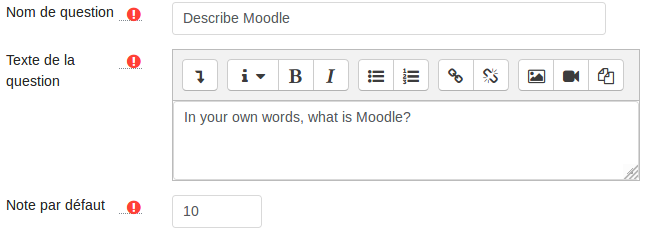
\includegraphics[scale=0.4]{../images/questionform_base.png}
    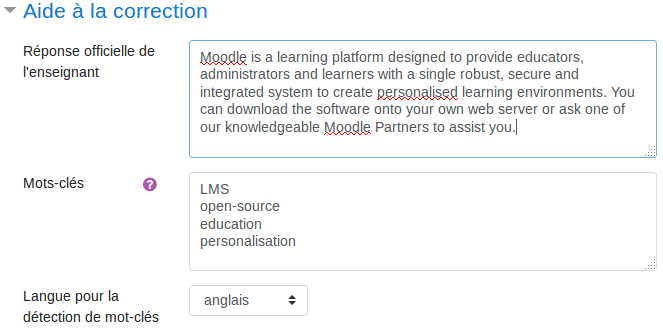
\includegraphics[scale=0.4]{../images/questionform_helper.png}
  \end{frame}
  
  \begin{frame}
  \frametitle{\insertsection}
  \alert{Exemple d'interface de correction}\vfill
  \begin{center}
    
\includegraphics[scale=0.6]{../images/questionform_correction.png}
  \end{center}
  \end{frame}
  
  \begin{frame}
    \frametitle{R\'esultats obtenus et limites de notre module de correction}
    \begin{block}{Pas de tests réels}
      \begin{itemize}
        \item Magda Fusaro est devenue Rectrice de l'UQAM
        \item Les \'evaluations dans mes cours au C\'egep n'ont pas de textes \`a d\'eveloppement
      \end{itemize}
    \end{block}
  
    \vfill


    \pause
  
    \begin{block}{La s\'eparation des mots peut \^etre inexacte}
      \begin{tabular}{lllll}
       \og aujourd'hui \fg{} & $\Rightarrow$ & \og aujourd \fg{} & $+$ & \og hui \fg{} 
        \\
        \og qu'autrui \fg{} & $\Rightarrow$ &  \og qu \fg{} & $+$ & \og autrui \fg{} 
        \\
        \og wasn't \fg{} &$\Rightarrow$ & \og wasn \fg{} &  $+$ & \og t \fg{} 
      \end{tabular}
    \end{block}
    \vfill

    \pause
    \begin{block}{Certains mots cl\'es peuvent \^etre mis en \'evidence plusieurs fois}
      \begin{itemize}
        \item \og aimera \fg{} $+$ \og aimerait \fg{} avec mot-cl\'e \og aimer \fg{}
      \end{itemize}
    \end{block}
  \end{frame}
  
  \begin{frame}
    \frametitle{\insertsection}
    \begin{block}{Am\'eliorations possibles}
      Mise en \'evidence configurable via l'interface

      \medskip
  
      Utilisation de la lemmatisation
  
      \medskip
  
      Comparaison des r\'eponses des \'etudiants pour plagiat
    \end{block}
  \end{frame}
  
  \section[Conclusion]{Conclusion}
  \begin{frame}
  \frametitle{\insertsection}
  \begin{block}{Mise en pratique de nouveaux outils}
  \begin{itemize}
    \item Tests unitaires
    \item Tests d'acceptation
    \item \LaTeX
  \end{itemize}
  \end{block}

  \vfill
  
  \begin{block}{Apprentissages}
  \begin{itemize}
    \item Analyser avant de se lancer
    \item G\'erer mon horaire
    \item \'Ecrire des rapports et des notes de cours
  \end{itemize}
  \end{block}
  \vfill
  \end{frame}
  
  \begin{frame}
  \begin{center}
  \Huge Merci!
  \end{center}

  \vfill

  \begin{center}
  \Huge Questions?
  \end{center}
  \vfill
  \end{frame}
\end{document}
